\chapter{Introduction}
\label{ch:intro}

\section{Introduction}

Teams of inexpensive rovers are being considered for planetary survey,
disaster-site inspection, agricultural monitoring and warehouse logistics,
precisely the places where fixed communication infrastructure is absent or
too costly to install. Such a team must organise itself: every few seconds
someone has to decide which rover takes which task, and that decision is only
as good as the information that reaches the decision maker. The information
travels over the rovers' own radios, in this project low-power ESP-NOW links
between ESP32-class microcontrollers. Each rover hears only a few nearby
teammates, and every link drifts as rovers move, batteries drain and terrain
gets in the way, so the communication network is a graph whose edges appear,
weaken and disappear from one control cycle to the next.

This report describes a complete pipeline for allocating tasks over that
moving graph and, equally important, an audit of how well each part works.
The pipeline first \emph{prunes} the graph to a small, reliable working
subgraph by solving a constrained optimisation problem written as a quadratic
unconstrained binary optimisation (QUBO), the native input of quantum and
quantum-inspired annealers. Once the graph has been pruned, a small graph
neural network (GNN) gives every rover a score. The scores depend on trust
values that the system learns online from how earlier tasks turned out, and a
greedy step then hands out the tasks while respecting how much work each rover
can take. We tested the pipeline in three settings, each more realistic than
the last. All of the numbers in this report come from a statistical simulator;
the other two settings are a physics simulation in Gazebo with ROS~2 and an
interactive 3D simulation engine that we built for this project.

\section{Overview of Dynamic Rover Networks}

We treat the fleet at control cycle $t$ as an undirected graph
$G_t=(V,E_t)$. Each vertex is a rover, and two rovers share an edge when they
are able to exchange packets during that cycle. Each edge carries normalised features describing
how much it is worth keeping (the trust and battery of its weaker endpoint, its
link quality, proximity, freshness, the criticality of the tasks at its ends
and its processing cost), and each rover carries its own trust, battery, load
and capability. These features feed both stages: they decide which edges
survive pruning and how information flows between neighbours during scoring
(Fig.~\ref{fig:intro:pruning}).

The hardware follows a three-tier mist--fog--cloud split. The rovers (mist)
sense and communicate; a gateway forwards telemetry to a Raspberry Pi (fog),
which maintains the graph, prunes it and runs inference within the cycle
deadline; and a laptop or server (cloud) hosts training and heavy
optimisation. Compute is scarcest exactly where decisions must be made
fastest, which shapes every design choice that follows.

\begin{figure}[htbp]
\centering
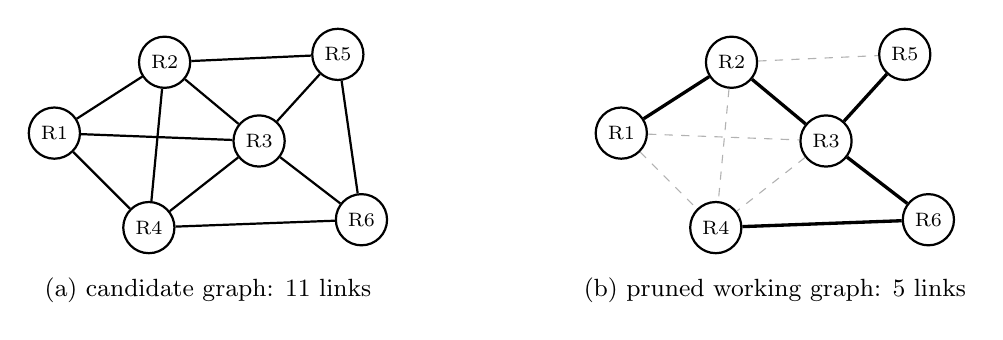
\begin{tikzpicture}[
  rover/.style={circle, draw, thick, fill=white, minimum size=6.5mm, inner sep=0pt, font=\scriptsize},
  weak/.style={gray!60, dashed},
  kept/.style={very thick},
]
\begin{scope}
\node[rover] (a) at (0,0) {R1};
\node[rover] (b) at (1.4,0.9) {R2};
\node[rover] (c) at (2.6,-0.1) {R3};
\node[rover] (d) at (1.2,-1.2) {R4};
\node[rover] (e) at (3.6,1.0) {R5};
\node[rover] (f) at (3.9,-1.1) {R6};
\foreach \u/\v in {a/b,a/c,a/d,b/c,b/d,c/d,b/e,c/e,c/f,d/f,e/f}{\draw[thick] (\u) -- (\v);}
\node[font=\small] at (1.95,-2.0) {(a) candidate graph: 11 links};
\end{scope}
\begin{scope}[xshift=7.2cm]
\node[rover] (a) at (0,0) {R1};
\node[rover] (b) at (1.4,0.9) {R2};
\node[rover] (c) at (2.6,-0.1) {R3};
\node[rover] (d) at (1.2,-1.2) {R4};
\node[rover] (e) at (3.6,1.0) {R5};
\node[rover] (f) at (3.9,-1.1) {R6};
\foreach \u/\v in {a/c,a/d,b/c,b/d,c/d,b/e}{\draw[weak] (\u) -- (\v);}
\foreach \u/\v in {a/b,b/c,c/e,c/f,d/f}{\draw[kept] (\u) -- (\v);}
\node[font=\small] at (1.95,-2.0) {(b) pruned working graph: 5 links};
\end{scope}
\end{tikzpicture}
\caption{The pruning idea: of the links in range (a), a small connected subset
is kept (b, solid) subject to link caps, a cost budget and connectivity of the
mission rovers.}
\label{fig:intro:pruning}
\end{figure}

\section{Challenges}

\begin{enumerate}[label=\arabic*.]
\item \textbf{Volatile links.} A link can get better, get worse or vanish as
rovers move, as interference changes and as distances grow. For this reason the
model also has to track how recently each link was heard.
\item \textbf{Hidden, drifting reliability.} Nobody can measure how reliable a
rover is. We can only estimate it from the tasks it was given, and which tasks
it was given depended on how much we trusted it in the first place.
\item \textbf{Scarce fog compute.} Message passing costs grow with the number
of edges, and the fog device has a small budget per cycle.
\item \textbf{Global constraints.} Whether the link caps, the processing
budget and the connectivity of the mission rovers are respected depends on the
kept graph as a whole. A rule that looks at one edge at a time has no way to
guarantee any of them.
\item \textbf{Solver reliability.} Even a correctly encoded problem does not
help if the solver gives back infeasible or weak answers, and this kind of
failure is only noticed when the answers are compared with an exact
solution.
\end{enumerate}

\section{Project Statement}

To design, implement and evaluate a pipeline for dynamic rover networks that
(i) prunes the communication graph every cycle with a constrained QUBO that
enforces degree, budget and connectivity constraints exactly; (ii) solves it
reliably and checks the solver against exact classical ground truth; (iii)
assigns tasks with a trust-aware GNN whose trust is learned online; (iv)
demonstrates the pipeline in a physics simulator and an interactive real-time
3D engine; and (v) reports honestly where the architecture pays off and where
simpler alternatives are as good or better.

\section{Objectives}

\begin{enumerate}[label=\arabic*.]
\item Formulate a constrained QUBO for dynamic graph pruning with exact,
flow-based connectivity, and verify it against an independent re-derivation
and exhaustive enumeration.
\item Explain why bit-level annealers fail on penalty-encoded QUBOs and build a
solver that reliably returns feasible, near-optimal edge sets.
\item Set up exact classical baselines so that each claim about a solver can
be checked against them.
\item Design a trust-weighted message-passing GNN with an online trust model,
cheap enough for a fog device.
\item Build a causal closed-loop simulator with a statistically sound
evaluation protocol, and a hostile automated test suite.
\item Deploy the pipeline in Gazebo with ROS~2 and in an interactive 3D
simulation engine with live tuning and side-by-side comparisons.
\end{enumerate}

\section{Scope}

The project covers the QUBO pruner, the trust-aware GNN and assignment, the
three-tier architecture, the test suite, the Gazebo and ROS~2 integration and
the 3D engine. Quantitative claims come from the statistical simulator, with
10 rovers for end-to-end experiments and 10 to 50 for scaling. Out of scope
are experiments on physical rovers (a four-rover testbed is designed but not
built), execution on quantum hardware (the QUBO matrix is exported but was not
run on a quantum processor) and channel-accurate radio modelling.

\section{Contributions}

\begin{enumerate}[label=\arabic*.]
\item A constrained QUBO for dynamic graph pruning in which connectivity is
enforced exactly by a single-commodity flow encoding (Chapter~\ref{ch:qubo}).
\item A quantitative account of the \emph{penalty barrier}: four serious
annealing samplers find the exact optimum on only 48 to 64\% of verifiable
instances, while a feasibility-projected annealer finds it on all of them
(Chapter~\ref{ch:solvers}).
\item Exact classical baselines showing that a direct mixed-integer program is
exact and about 100 times faster, which fixes the QUBO's honest role as a
hardware-target encoding (Chapter~\ref{ch:exact}).
\item A trust-aware assignment layer that beats a trust-only baseline by 8.1
points of mission success with a confidence interval excluding zero
(Chapters~\ref{ch:gnn} and~\ref{ch:results}).
\item A causal evaluation with constraint-aware baselines, a ten-level
constraint-pressure sweep, and an audit that caught a silent budget
relaxation in the project's own earlier results
(Chapters~\ref{ch:sim}--\ref{ch:results}).
\item Two deployments: a containerised Gazebo Harmonic and ROS~2 Jazzy world
(Chapter~\ref{ch:gazebo}) and an interactive 3D engine with provably
collision-free motion and a seven-draw-call renderer (Chapter~\ref{ch:engine}).
\end{enumerate}

\section{Organization of the Report}

Chapter~\ref{ch:background} surveys the background and related work, and
Chapter~\ref{ch:arch} presents the system model. Chapters~\ref{ch:qubo}
to~\ref{ch:exact} form the optimisation core: formulation, solvers and exact
baselines. Chapter~\ref{ch:gnn} covers trust-aware inference and assignment,
Chapter~\ref{ch:sim} the simulator and methodology, Chapter~\ref{ch:verify}
verification, and Chapter~\ref{ch:results} the results.
Chapters~\ref{ch:gazebo} and~\ref{ch:engine} describe the Gazebo integration
and the 3D engine, and Chapter~\ref{ch:conclusion} concludes.
